

\section{Histogram Methods}

Histogram methods go back to \citet{salzburg}. To reduce the computational cost, one can compute a certain quantity at a given temperature and then extrapolate the result to other temperatures. This is only possible if the temperature dependence is known. In the case of canonical variables the dependence is given by the Boltzmann factor. As a start, the partition function is reformulated as a sum over all possible energies instead of over all possible configurations:
\begin{equation}
Q\kl{T} = \frac{1}{Z_T}\sum_E{Q\kl{E} p_T\kl{E}}\text{\hspace{0.2cm}with } Z_T=\sum_E{p_T\kl{E}}
\label{eq:part_fun_over_energy}
\end{equation}
where $p_T\kl{E} \equiv g\kl{E} e^{-\frac{E}{k_BT}}$ with $g\kl{E}$ being the \emph{density of states} (i.e. the number of states with energy $E$). This takes into account the fact that more configurations can have the same energy. The goal is to compute the quantity $Q$ at another temperature $T^*$:  $Q\kl{T^*} = \frac{1}{Z_T^*}\sum_E{Q\kl{E} p_T^*\kl{E}}$. The density of states contains all the information needed. Using the definition of $g\kl{E}$ yields 
$$p_{T^*}\kl{E}=g\kl{E}e^{-\frac{E}{k_BT^*}} \underbrace{=}_{\text{def. of $g\kl{E}$}}  p_T\kl{E}exp\ekl{-\frac{E}{k_BT^*}+\frac{E}{k_BT}}
$$
and with $f_{T,T^*}\kl{E}\equiv exp\ekl{-\frac{E}{k_BT^*}+\frac{E}{k_BT}} $ one finally obtains
\begin{equation}
Q\kl{T^*} = \frac  { \sum_E {Q\kl{E} p_T\kl{E} f_{T,T^*}\kl{E} }}   {  \sum_E  p_T\kl{E} f_{T,T^*}\kl{E} }.
\label{eq:histo_average}
\end{equation}
We have now obtained an expression for the quantity $Q$ at the temperature $T^*$ without having to measure any distribution at temperature T, since $f_{T,T^*}$ are known scalars. The drawback of this method is that the values of $Q\kl{E}$ are sampled around the maximum of $p_T\kl{E}$, which  converges to a delta distribution for large systems. This means that if $T$ and $T^*$ are not very close, the statistics are very poor, and results will be inaccurate or  even wrong. One possible solution consists of interpolating data from several temperatures (multi-canonical method) but this involves calculations for many temperatures, which is also not efficient for large systems. Another solution to this problem has been presented in \citet{oliveira} and will be also treated in this chapter.
\subsection{Broad Histogram Method}
The aim of the broad histogram method (BHMC) is to directly calculate the density of states. It obtains the function $g(E)$ through a stochastic process. The density of states increases very steeply (exponentially) with energy $E$, since the number of possible configurations increases with higher energy. A plain random walk through phase space would also have the problem that it would explore only the regions with high energies. To explore all the regions equally (with respect to the energy) we can create a Markov chain in which the number of processes that increase the energy by $\Delta E$ (we shall call this number $N_{up}$) and the number of processes that decrease the energy ($N_{down}$) fulfill an equivalent condition to detailed balance to reach a homogeneous steady state:

\begin{equation}
g\kl{E+\Delta E} N_{down}\kl{E+\Delta E} = g\kl{E} N_{up}\kl{E}.
\label{eq:detailed_balance_broad_histo}
\end{equation}
The motion (in phase space) towards higher energies can then be penalized with Metropolis-like dynamics:
\begin{itemize}
\item Choose a new configuration
\item If the new energy is lower, accept the move
\item If the new energy is higher then accept with probability $\frac{N_{down}\kl{E+\Delta E}}{N_{up}\kl{E}}$
\end{itemize}
However, we haven't obtained the function $g\kl{E}$ yet. Therefore we will take the logarithm of Eq. \eqref{eq:detailed_balance_broad_histo} and divide by $\Delta E$


$$
\log \ekl{g\kl{E+\Delta E} } - \log \ekl{g\kl{E} } = - \log \ekl{N_{up}\kl{E} }  - \log \ekl{N_{down}\kl{E+\Delta E} } 
$$
\begin{equation}
\Rightarrow
\pder{\log \ekl{g\kl{E} } }{E} = \frac{1}{\Delta E}\log \ekl{\frac{N_{up}\kl{E}}{N_{down}\kl{E+\Delta E}} }  
\end{equation}
which we can numerically integrate to obtain $g\kl{E}$. Estimates of $N_{up}$ and $N_{down}$ can be obtained by checking if a change of state at each site would increase or decrease the energy. 



\vspace{0.1cm}
\noindent
\begin{minipage}{\textwidth}
\begin{minipage}{.48\textwidth}
  \centering
  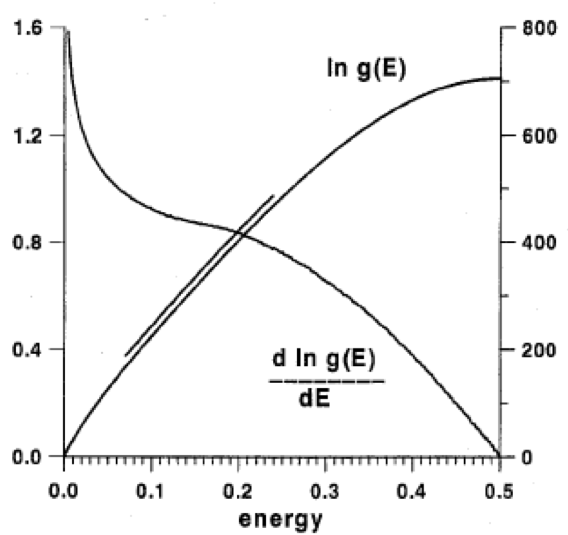
\includegraphics[width = \textwidth]{pics/broad_histo_1}
  \captionof{figure}{Example for the density of states for the Ising model}
  \label{fig:broad_histo_1}
\end{minipage}\hfill
\begin{minipage}{.48\textwidth}
  \centering
  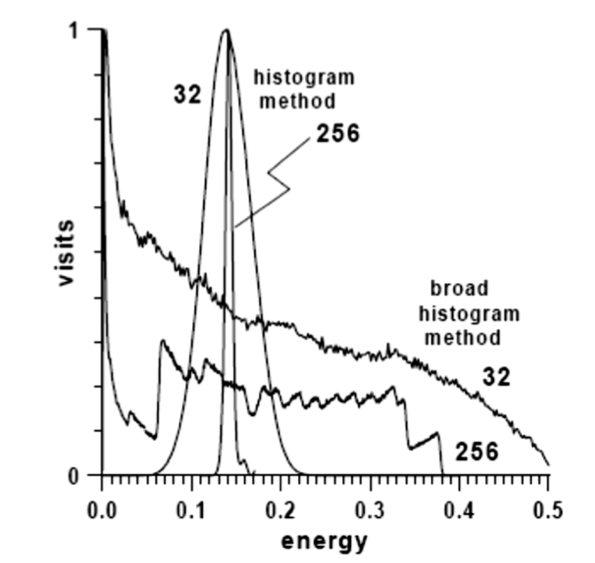
\includegraphics[width = \textwidth]{pics/broad_histo_2}
  \captionof{figure}{Number of visits done in the phase space against the energy.}
  \label{fig:broad_histo_2}
\end{minipage}
\end{minipage}
\vspace{0.1cm}




\vspace{0.1cm}
\noindent
\begin{minipage}{\textwidth}
\begin{minipage}{.48\textwidth}
While moving through phase space one can not only accumulate the values of $N_{up}$ and $N_{down}$, but also keep the values for any quantity $Q\kl{E}$. Finally one can compute
$$
Q\kl{T} = \frac  {\sum_E {Q\kl{E}g\kl{E}e^{-\frac{E}{k_BT}}}  }  {\sum_E {g\kl{E}e^{-\frac{E}{k_BT}}} }
$$
Knowing $g\kl{E}$ one can now calculate quantities at any temperature.
\end{minipage}\hfill
\begin{minipage}{.48\textwidth}
  \centering
  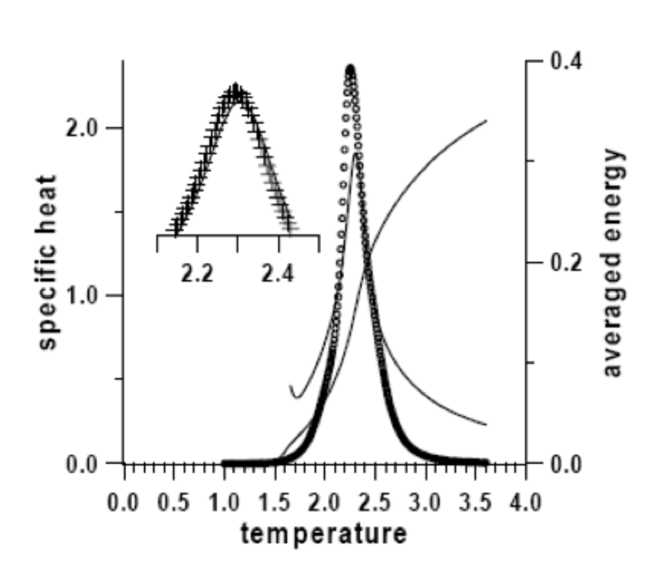
\includegraphics[height=140pt]{pics/broad_histo_3}
 \captionof{figure}{\small The continuous line is the analytic solution of the specific heat for a 32x32 lattice. The crosses represents the result of the BHMC and the circles are the result for the usual histogram.}
  \label{fig:broad_histo_3}
\end{minipage}
\end{minipage}
\vspace{0.1cm}




\subsection{Flat Histogram Method}

This is another method, proposed by Wang, to obtain a flat distribution of visits in energy space. The basic algorithm works as follows:
\begin{itemize}
\item Start with $g\kl{E}=1$ and set $f\equiv E$.
\item Make MC update with $p(E)=1/g(E)$.
\item If the attempt is successful at $E$: $g(E)=f\cdot g(E)$.
\item Obtain a histogram of the energies $H(E)$.
\item If $H(E)$ is flat enough, then $f\equiv \sqrt{f}$.
\item Stop when $f\le 10^{-8}$.
\end{itemize}

Note that choosing the probability as $1/g(E)$ in the second step implies that for higher configuration density at energy $E$, the choosing probability decreases. Therefore the method tends to go towards energies with fewer configurations. At this point the function has to be corrected by updating the value of $g$ and the energy $E$. Once a histogram has been obtained one can increase the precision by decreasing $f$, e.g. by dividing it by two. The ``flatness'' of the histogram can be measured as the ratio of the minimum to the maximum value. For further details, see the \emph{Wang-Landau} algorithm.

\subsection{Umbrella sampling}

This technique was developed and proposed in \citet{torrie}. The aim is to overcome the problem of the lack in ergodicity for certain energy landscapes. As an example, in the Ising model the system could have difficulties in jumping from a positive to a negative magnetization (or vice versa) if the system is very large. The basic idea is to multiply transition probabilities with a function that is large at the free energy barrier and later remove this correction in the averaging step.
\begin{equation}
\tilde{p} \kl{C} = \frac{w\kl{C} e^{-\frac{E\kl{C}}{k_BT}}}{\sum_C{w\kl{C} e^{-\frac{E\kl{C}}{k_BT}}}}
\text{ \hspace{0.1cm} with \hspace{0.1cm} }
\avkl{A} = \frac{\avkl{A/w}_w}{\avkl{1/w}_w}.
\label{eq:torrie}
\end{equation}

\vspace{0.2cm}
\noindent
Summarizing, some of the most common techniques related to the histogram methods are

\begin{itemize}
\item Wang-Landau method 
\item Multiple histogram method
\item Multicanonical MC
\item Flat Histogram method
\item Umbrella sampling
\end{itemize}





